% !TeX root = ../tlmgr-intro-zh-cn.tex
\section*{前\quad 言}
\addcontentsline{toc}{section}{前言}

这个文档是对 \href{https://mirrors.ctan.org/info/tlmgrbasics/doc/tlmgr.pdf}{\texttt{texdoc tlmgr}} 的翻译以及补充. 由于翻译水平与专业知识有限, 文档中有一些词汇和语句翻译的并不好, 如果您有更好的翻译或者纠正我的错误, 可以在该项目处提出 \href{https://github.com/syvshc/tlmgr-intro-zh-cn/issues}{issue} 或者 \href{https://github.com/syvshc/tlmgr-intro-zh-cn/pulls}{PR}. 

\tlmgr 管理着 \tl 的安装, 包括软件包以及配置选项. 如果还没有安装 \tl, 可以参考 \href{https://mirrors.ctan.org/info/install-latex-guide-zh-cn/install-latex-guide-zh-cn.pdf}{install-latex-guide-zh-cn} 与 \href{https://www.tug.org/texlive/doc/texlive-zh-cn/texlive-zh-cn.pdf}{texlive-zh-cn} 进行安装. 

\tl 是由一些最高级别的\textbf{安装方案} (schemes) 构成的, 每一种方案中包含一些\textbf{集合} (collections) 和\textbf{软件包} (packages), 而每一个集合中也包含了一些软件包, 软件包中包含了一些可以看到的文件. 在安装 \tl 的时候, 我们可以选择在不同的级别来进行安装和管理. 比如在安装的时候可以只选则安装最小的安装方案 \texttt{minimal scheme (plain only)}, 以及一部分语言和功能的集合, 比如 \texttt{Chinese} 与 \texttt{LaTeX additional packages}

\begin{center}
    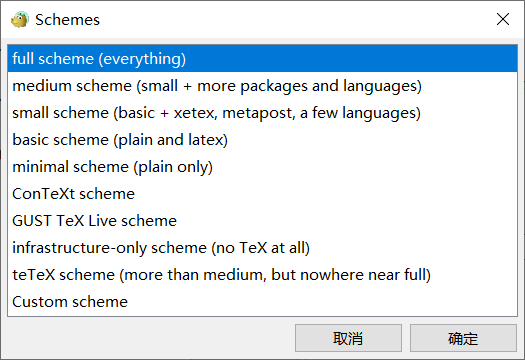
\includegraphics[height=4cm]{scheme.png} \quad 
    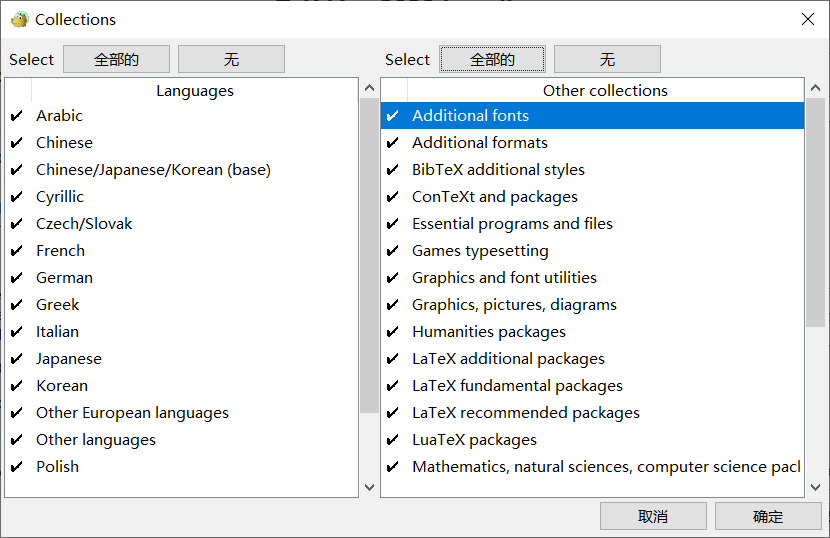
\includegraphics[height=4cm]{collection.png}
    \captionof{figure}{Schemes 与 collections}
\end{center}

使用 \tlmgr 管理这些安装方案, 集合和软件包是很有必要的, 但是 \href{https://www.tug.org/texlive/doc/tlmgr.html}{\tlmgr 官方文档} 过于冗长, 有很多一般用户接触不到的功能, 在这里将它简化, 拿出一些比较基础使用的命令来介绍. 

\tlmgr 也提供了图形界面: \texttt{tlshell}, \texttt{tlcockpit}, 在 Mac 上, 有 \tl{} Utility, 这些都需要启动另外的程序, 这篇简介只介绍命令行下的使用, 关于图形界面的使用可以看
\begin{center}
    \url{https://tug.org/texlive/doc/tlmgr.html#GUI-FOR-TLMGR}.
\end{center}